% LaTeX Poster vim:ts=2 sw=2
% 
\documentclass[final,xcolor={svgnames}]{beamer}

\newcommand{\leftlogo}{
\includegraphics[height=1.5in]{figures/stanford.pdf}}
%\newcommand{\rightlogo}{{\Huge$\mathbb{P}\lambda$}}
\newcommand{\rightlogo}{
\includegraphics[height=1.5in]{figures/nlp-logo.pdf}}
\newcommand{\leftfooter}{NLP at Stanford University}
%\newcommand{\leftfooter}{$\mathbb{P}\lambda$ at Stanford University}
\newcommand{\centerfooter}{\texttt{http://bit.ly/codalab-lense}}
\newcommand{\rightfooter}{\texttt{\{keenon,chaganty,pliang,manning\}@cs.stanford.edu}}
\mode<presentation>{\usetheme{I6pd2}}

\usepackage{grffile}
\usepackage[english]{babel}
\usepackage[latin1]{inputenc}
\usepackage{subfigure}

\boldmath{}
\usepackage{graphicx}
\usepackage[orientation=landscape,size=a1,scale=1.4]{beamerposter}
% change list indention level
% \setdefaultleftmargin{3em}{}{}{}{}{}
%\usepackage{snapshot} % will write a .dep file with all dependencies, allows for easy bundling

\usepackage{array,booktabs,tabularx}
\newcolumntype{Z}{>{\centering\arraybackslash}X} % centered tabularx columns


%\listfiles

%%%%%%%%%%%%%%%%%%%%%%%%%%%%%%%%%%%%%%%%%%%%%%%%%%%%%%%%%%%%%%%%%%%%%%%%%%%%%%%%%%%%%%
\graphicspath{{../figures/}}
\usepackage[nodefinetheorems]{scabby}
\usepackage{scabby-diag}

\providecommand{\muh}{\hat{\mu}}
\providecommand{\yh}{\hat{y}}

 
\title{On-the-Job Learning with Bayesian Decision Theory}
\author{Keenon Werling \and Arun Tejasvi Chaganty \and Percy Liang \and Christopher D. Manning} 
\institute[Stanford University]{Department of Computer Science\\ Stanford University}
%\date[Sep. 8th, 2009]{Sep. 8th, 2009}

%%%%%%%%%%%%%%%%%%%%%%%%%%%%%%%%%%%%%%%%%%%%%%%%%%%%%%%%%%%%%%%%%%%%%%%%%%%%%%%%%%%%%%
% You wlll have to manually set the height of the page
% 105cm is good for A0. 52 for A2, 22 for A3
\newlength{\columnheight}
\setlength{\columnheight}{52cm}
%%%%%%%%%%%%%%%%%%%%%%%%%%%%%%%%%%%%%%%%%%%%%%%%%%%%%%%%%%%%%%%%%%%%%%%%%%%%%%%%%%%%%%
\begin{document}

% Everything is contained in this frame
\begin{frame}
  % Standard two column layout
  \begin{columns}
    %%%%%%%%%%%%%%%%%%%%%%%%%%%%%%%%%%%%%%%%%%%%%%%%%%%%%%%%%%%%%%%%%%%%%%%%%%%%%%%%%%%%%%
    % Column 1
    \begin{column}{.32\textwidth}
      \begin{beamercolorbox}[center,wd=\textwidth]{postercolumn}
        \begin{minipage}[T]{.95\textwidth}  % tweaks the width, makes a new \textwidth
          \parbox[t][\columnheight]{\textwidth}{% must be some better way to set the the height, width and textwidth simultaneously
            % Since all columns are the same length, it is all nice and tidy.  You have to get the height empirically
            % ---------------------------------------------------------%
            % fill each column with content            
            \vfill
\begin{block}{Big picture}
  \begin{center}
  {\large How do you deploy a high accuracy classifier starting with zero training examples?}\\
  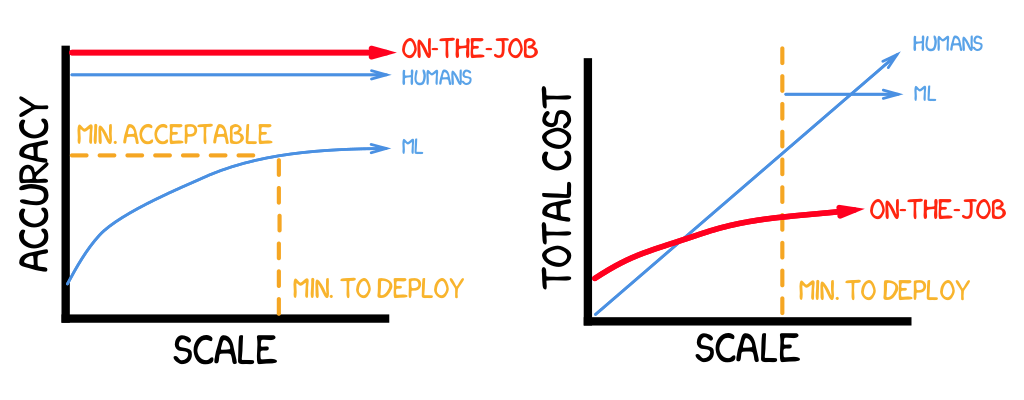
\includegraphics[width=0.8\columnwidth]{graph}
  \end{center}

\end{block}
\vfill

\begin{block}{What is on-the-job learning?}
  \begin{itemize}
    \item 
  \textbf{On-the-job learning} allows a system to query the crowd for labels on the uncertain parts of an input as it arrives \textbf{before} making a prediction.

%  \begin{center}
%    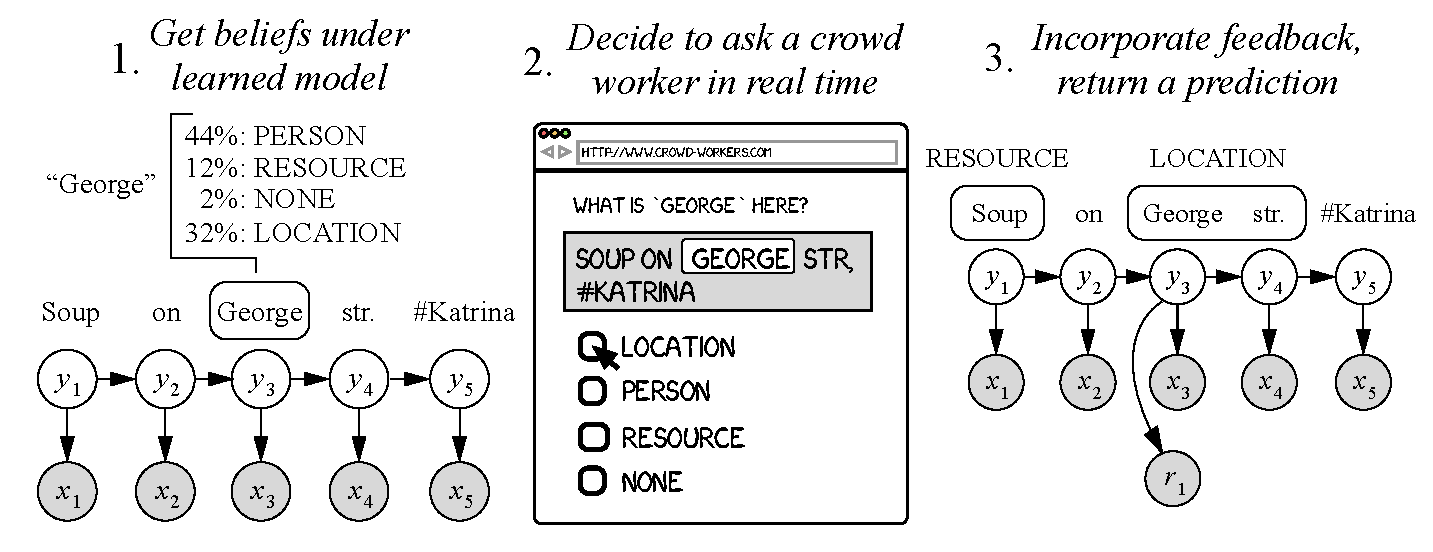
\includegraphics[width=0.8\columnwidth]{intro-banner}
%  \end{center}

    \item Can \textbf{maintain accuracy on difficult examples} by asking the crowd for assistance.
    \item \textbf{Reduces costs} on simpler examples by learning a better prediction model online (on-the-job).
    \item User specifies a base prediction model and how to trade off accuracy, cost and latency. 
    \item System optimizes for utility using ideas from game playing and Bayesian decision theory.
  \end{itemize}
\end{block}
\vfill

\begin{block}{Related work}
  \begin{tabular}{p{0.54\columnwidth} p{0.39\columnwidth}}
    \textbf{Area} & \textbf{Paradigm} \\ \midrule
    \textbf{Online active learning}
      chooses the most informative examples to label \emph{after} classification. 
      Impossible to maintain high accuracy initially.
      & 
      \begin{center}
      \tikz{
      \node[draw, fill=palette2, rectangle, scale=0.7] (inp) {\textsc{Input}};
      \node[draw, fill=palette3, rectangle, right, scale=0.7] (pred) at ($(inp.east)$) {\textsc{Predict}};
      \node[draw, fill=palette5, rectangle, right, scale=0.7] (label) at ($(pred.east)$) {\textsc{Label}};
      \node[draw, fill=palette1, rectangle, right, scale=0.7] (learn) at ($(label.east)$) {\textsc{Learn}};
      }
      \end{center}
      \\
      %Input, Predict, Label, Learn \\
    \textbf{Active classification} 
    learns a static policy from a labelled dataset to choose features to query at test time.
      & 
      \begin{center}
      \tikz{
      \node[draw, fill=palette2, rectangle, scale=0.7] (inp) {\textsc{Input}};
      \node[draw, fill=palette5, rectangle, right, scale=0.7] (label) at ($(inp.east)$) {\textsc{Label}$^*$};
      \node[draw, fill=palette3, rectangle, right, scale=0.7] (pred) at ($(label.east)$) {\textsc{Predict}};
%      \node[draw, fill=palette1, rectangle, right, scale=0.7] (learn) at ($(pred.east)$) {\phantom{Learn}};
      }
      \end{center}
      \\
    \textbf{On-the-job learning}
    combines advantages of both the above methods. Note,
Legion:AR \citep{lasecki2013real} studied the user interface
      aspects of on-the-job learning, while we study the machine learning
      aspects of it.
      & 
      \begin{center}
      \tikz{
      \node[draw, fill=palette2, rectangle, scale=0.7] (inp) {\textsc{Input}};
      \node[draw, fill=palette5, rectangle, right, scale=0.7] (label) at ($(inp.east)$) {\textsc{Label}};
      \node[draw, fill=palette3, rectangle, right, scale=0.7] (pred) at ($(label.east)$) {\textsc{Predict}};
      \node[draw, fill=palette1, rectangle, right, scale=0.7] (learn) at ($(pred.east)$) {\textsc{Learn}};
      }
      \end{center}
      \\
  \end{tabular}


  %\begin{itemize}
  %  \item Legion:AR \citep{lasecki2013real} study the user interface
  %    aspects of on-the-job learning, while we study the machine learning
  %    aspects of it.



  %  \item \textbf{Online active learning}: The key distinction from
  %    online active learning is that in on-the-job learning, (noisy
  %    partial) labels are obtained \emph{before} a prediction is made.
  %    \todo{figure}.
  %  \item \textbf{Active classification}: Active classification algorithms learns a static policy from a labelled dataset for when certain features should be queried which does not change at test time, whereas on-the-job learning continuously updates itself, 
  %\end{itemize}
\end{block}
\vfill


          }
        \end{minipage}
      \end{beamercolorbox}
    \end{column}

    %%%%%%%%%%%%%%%%%%%%%%%%%%%%%%%%%%%%%%%%%%%%%%%%%%%%%%%%%%%%%%%%%%%%%%%%%%%%%%%%%%%%%%
    % Column 2
    \begin{column}{.32\textwidth}
      \begin{beamercolorbox}[center,wd=\textwidth]{postercolumn}
        \begin{minipage}[T]{.95\textwidth} % tweaks the width, makes a new \textwidth
          \parbox[t][\columnheight]{\textwidth}{% must be some better way to set the the height, width and textwidth simultaneously
            % Since all columns are the same length, it is all nice and tidy.  You have to get the height empirically
            % ---------------------------------------------------------%
            % fill each column with content
            \begin{block}{Example: named entity recognition on tweets}
  \begin{center}
    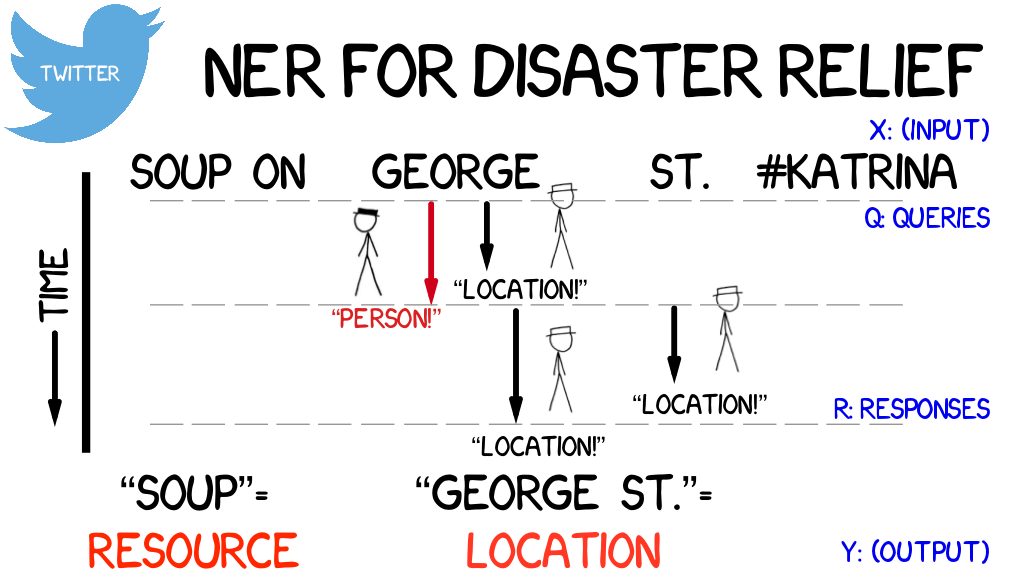
\includegraphics[width=0.79\columnwidth]{soup-example.png}
  \end{center}
\end{block}
\vfill

\begin{block}{How marginals evolve after incorporating responses}
  \begin{center}
    \includegraphics[width=0.79\columnwidth]{behavior-poster}
  \end{center}
\end{block}
\vfill

\begin{block}{Approximating utility with MCTS}
  \splitcolumn{
    \begin{center}
      \includegraphics[width=0.89\columnwidth]{mcts_poster}
    \end{center}
  }{
  \begin{itemize}
    \item \textbf{Stochastic game} between system and crowd.
    \item \textbf{States} capture time, queries in flight and received responses.
    \item \textbf{Actions} are querying for a label, waiting or returning current best guess.
  \end{itemize}
  }
  \begin{itemize}
    \item The system chooses actions that \textbf{maximize utility}.
    \item Approximated by Markov Chain Tree Search (MCTS) with progressive widening, using an environment model.
  \begin{align*}
    \label{eqn:dynamics}
  %p(\by, \br, \bt \mid \bx, \bq) \eqdef \p(\by \given \bx) \prod_{i=1}^k \presp(r_i \mid \bx, \by, q_i) \ptime(t_i \mid \bx, \by, q_i, s_i).
  \underbrace{p(\by, \br, \bt \given \bx, \bq, \bs)}_{\textrm{environment model}} \eqdef \underbrace{\p(\by \given \bx)}_{\textrm{prediction}} \prod_{i=1}^k \underbrace{\presp(r_i \mid y_{q_i})}_{\textrm{annotator noise}} \underbrace{\ptime(t_i \mid s_i)}_{\textrm{latency}}.
  \end{align*}
    \item Use human-labelled examples as training data to learn the model.
  \end{itemize}

\end{block}
\vfill

%\begin{block}{Model: a stochastic game between the system and the crowd.}
%  \begin{itemize}
%    \item The game starts with the system receiving input $\bx$ and ends when the system turns in a set of labels $\by = (y_1, \ldots, y_n)$. 
%    \item During the system's turn, the system may choose a query action $q \in \{1, \ldots, n\}$ to ask the crowd to label $y_q$. The system may also choose 
%the wait action ($q = \acwait$) to wait for the crowd to respond to a pending query
%or
%the return action ($q = \acret$) to terminate the game and return its prediction given responses received thus far.
%\item
%The system can make as many queries in a row (i.e.\ simultaneously) as it wants, before deciding to wait or turn in.
%\item When the wait action is chosen, the turn switches to the crowd, which provides a response $r$ to one pending query, and advances the game clock by the time taken for the crowd to respond. The turn then immediately reverts back to the system.
%\item When the game ends (the system chooses the return action), the system evaluates a utility that depends on the accuracy of its prediction,
%the number of queries issued and the total time taken.
%\item The system should choose query and wait actions to
%maximize the utility of the prediction eventually returned.
%\item \textbf{Utility} trades off the accuracy of the MAP estimate according to the model's best guess of $\by$ incorporating all responses received by time $\tau$ and the cost of making queries: a (monetary) cost $\weightmoney$ per query made and penalty of $\weighttime$ per unit of time taken.
%\begin{align}
%  \label{eqn:utility}
%  U(\sigma) &\eqdef \text{ExpAcc}(p(\by \given \bx, \bq, \bs, \br, \bt)) - (n_\text{Q} \weightmoney + \now \weighttime), \\
%  \text{ExpAcc}(p) &= \E_{p(\by)}[\text{Accuracy}(\arg\max_{\by'} p(\by'))],
%\end{align}
%\item \textbf{Environmnet model}
%\begin{align}
%  \label{eqn:dynamics}
%%p(\by, \br, \bt \mid \bx, \bq) \eqdef \p(\by \given \bx) \prod_{i=1}^k \presp(r_i \mid \bx, \by, q_i) \ptime(t_i \mid \bx, \by, q_i, s_i).
%p(\by, \br, \bt \given \bx, \bq, \bs) \eqdef \p(\by \given \bx) \prod_{i=1}^k \presp(r_i \mid y_{q_i}) \ptime(t_i \mid s_i).
%\end{align}
%
%  \end{itemize}
%\end{block}
%
%\begin{block}{}
%  \begin{center}
%    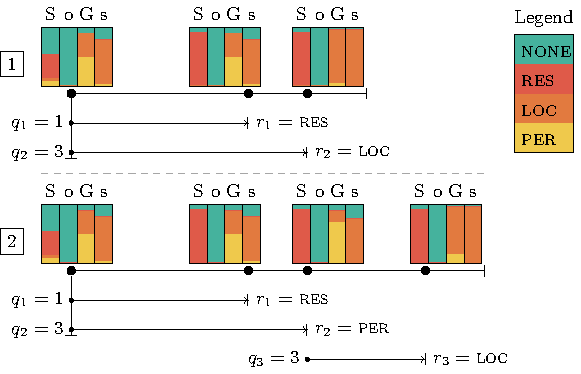
\includegraphics[width=0.59\columnwidth]{behavior}
%    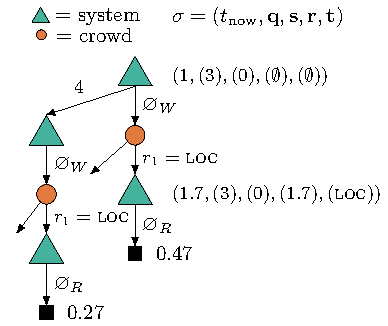
\includegraphics[width=0.39\columnwidth]{mcts_simple}
%  \end{center}
%\end{block}
%
%\begin{block}{Learning and inference}
%  \begin{itemize}
%    \item TODO insert algorithm.
%  \end{itemize}
%\end{block}


          }
          % ---------------------------------------------------------%
          % end the column
        \end{minipage}
      \end{beamercolorbox}
    \end{column}
    % ---------------------------------------------------------%
    % end the column

    %%%%%%%%%%%%%%%%%%%%%%%%%%%%%%%%%%%%%%%%%%%%%%%%%%%%%%%%%%%%%%%%%%%%%%%%%%%%%%%%%%%%%%
    % Column 3
    \begin{column}{.32\textwidth}
      \begin{beamercolorbox}[center,wd=\textwidth]{postercolumn}
        \begin{minipage}[T]{.95\textwidth} % tweaks the width, makes a new \textwidth
          \parbox[t][\columnheight]{\textwidth}{% must be some better way to set the the height, width and textwidth simultaneously
            % Since all columns are the same length, it is all nice and tidy.  You have to get the height empirically
            % ---------------------------------------------------------%
            % fill each column with content
            
\begin{block}{Named Entity Recognition (CoNLL 2003)}
\begin{table}[t]
  {\small
%% NER 
\begin{tabular}{l r r r r r r }
%  \multicolumn{7}{c}{Named Entity Recognition}  \\
      \textbf{System} & \textbf{Latency/tok} & \textbf{Qs/tok} & \textbf{PER F$_1$} & \textbf{LOC F$_1$} & \textbf{ORG F$_1$} & \textbf{F$_1$}
    \\ \hline
    1-vote & 467 ms & 1.0 & 90.2 & 78.8 & 71.5 & 80.2
      \\ %\hline
    3-vote & 750 ms & 3.0 & 93.6 & 85.1 & 74.5 & 85.4
        \\ %\hline
    5-vote & 1350 ms & 5.0 & \textbf{95.5} & 87.7 & 78.7 & 87.3 
        \\ \hline
    Online & n/a & n/a & 56.9 & 74.6 & 51.4 & 60.9
        \\    %\hline
    Threshold & 414 ms & 0.61 & 95.2 & \textbf{89.8} & 79.8 & 88.3
        \\ %\hline
    \textbf{LENSE} & \textbf{267 ms} & \textbf{0.45} & 95.2 & 89.7 & \textbf{81.7} & \textbf{88.8} 
\end{tabular}
}
%\caption{Results on NER (CoNLL 2003) comparing latencies, queries per token (Qs/tok) and per-class \fone{} scores.}
\label{tbl:results}
\end{table}

  \begin{center}
    \colorbox{white}{
    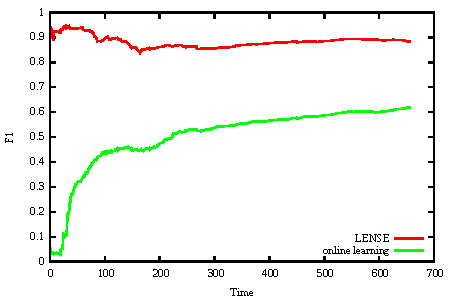
\includegraphics[width=0.45\columnwidth]{ner_2_class/f1_plot/f1_vs_time.pdf}
    }
    \colorbox{white}{
    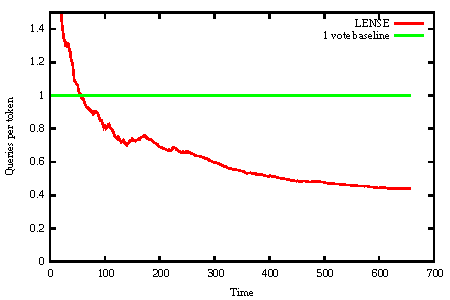
\includegraphics[width=0.45\columnwidth]{ner_2_class/cost_plot/cost_vs_time.pdf}
    }
  \end{center}

  \begin{exampleblock}{Takeaway}
      On-the-job learning is capable of making consistently accurate predictions while reducing annotation costs.
  \end{exampleblock}
\end{block}
\vfill

\begin{block}{Sentiment}
    \begin{minipage}[t]{.43\columnwidth}
      \colorbox{white}{
      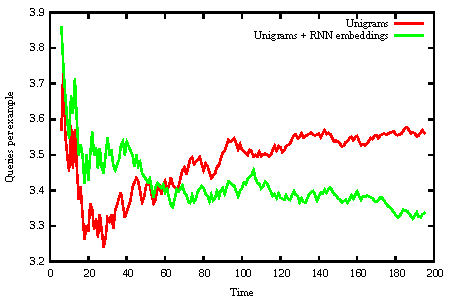
\includegraphics[width=\textwidth]{sentiment_cost_per_token_vs_time/cost_per_token_vs_time.pdf}
      }
    \end{minipage}
    \quad
    \begin{minipage}[t]{.45\columnwidth}
      \begin{tabular}[b]{l  r  r  r  r}
          %\hline
          \textbf{System} & \textbf{Latency} & \textbf{Qs/ex} & \textbf{Acc.} \\ \hline
          5-vote & 13.5 s & 5.00 & 98.7 \\ %\hline
          \multicolumn{5}{c}{\textsc{unigrams}} \\ \hline
          Online & n/a & n/a & 78.1 \\ %\hline
          Threshold & 10.9 s & 2.99 & 95.9 \\ %\hline
          \textbf{LENSE} & 11.7 s & 3.48 & 98.6 \\ %\hline
          \multicolumn{5}{c}{\textsc{rnn}} \\ \hline
          Online & n/a & n/a & 85.0 \\ %\hline
          Threshold & 11.0 s & 2.85 & 96.0 \\ %\hline
          \textbf{LENSE} & 11.0 s & 3.19 & 98.6 \\% \hline
      \end{tabular}
    \end{minipage}%

  \begin{exampleblock}{Takeaway}
      On-the-job learning will maintain accuracy even if the model lacks the capacity to.
  \end{exampleblock}
\end{block}
\vfill

\begin{block}{Conclusions and Future Work}
  \begin{itemize}
    \item Consider on-the-job learning to get accurate labels on your
      next project for cheap. 
    \item Easy to use open-source implementation, LENSE, available!
    \item Future directions include improving confidence estimation, 
      learning from measurements and more applications.
  \end{itemize}
\end{block}
\vfill


          }
          % ---------------------------------------------------------%
          % end the column
        \end{minipage}
      \end{beamercolorbox}
    \end{column}
    % ---------------------------------------------------------%
    % end the column

  \end{columns}
  \vskip2ex
\end{frame}

\end{document}

